\chapter{A Wider View: Models of Other Supernova Remnants}\label{chp:chp6}

%\begin{flushright}
%  {\em QUOTE GOES HERE }\\
%
%\ \
%
%\normalsize
%{AUTHOR}  
%\end{flushright}


\noindent{FIRST PARAGRAPH}

\section{Introduction}

\setlength{\tabcolsep}{7pt}
\begin{table}
%	\begin{minipage}{180mm}
	\centering
	\caption{Details of the archival data for SN~1980K, SN~1993J and Cas~A.}
	\label{tb:data}
  	\begin{tabular}{@{} ccccccccl @{}}
    	\hline
	Date & Age & Telescope  & Inst & $\lambda_{min}$ & $\lambda_{max}$ & Res. & Res. & Reference \\
	& (days) & & &(\AA) & (\AA)& (\AA) & Power\\
	\hline
31 Jul 1988 & 524 & AAT & FORS & 5500 & 10190 & 20 & & \citet{Spyromilio1991} \\

    \hline
  \end{tabular}
%\end{minipage}
\end{table}


\setlength{\tabcolsep}{12pt}

\section{SN~1980K}

\subsection{Smooth Models}
\begin{figure}
\centering
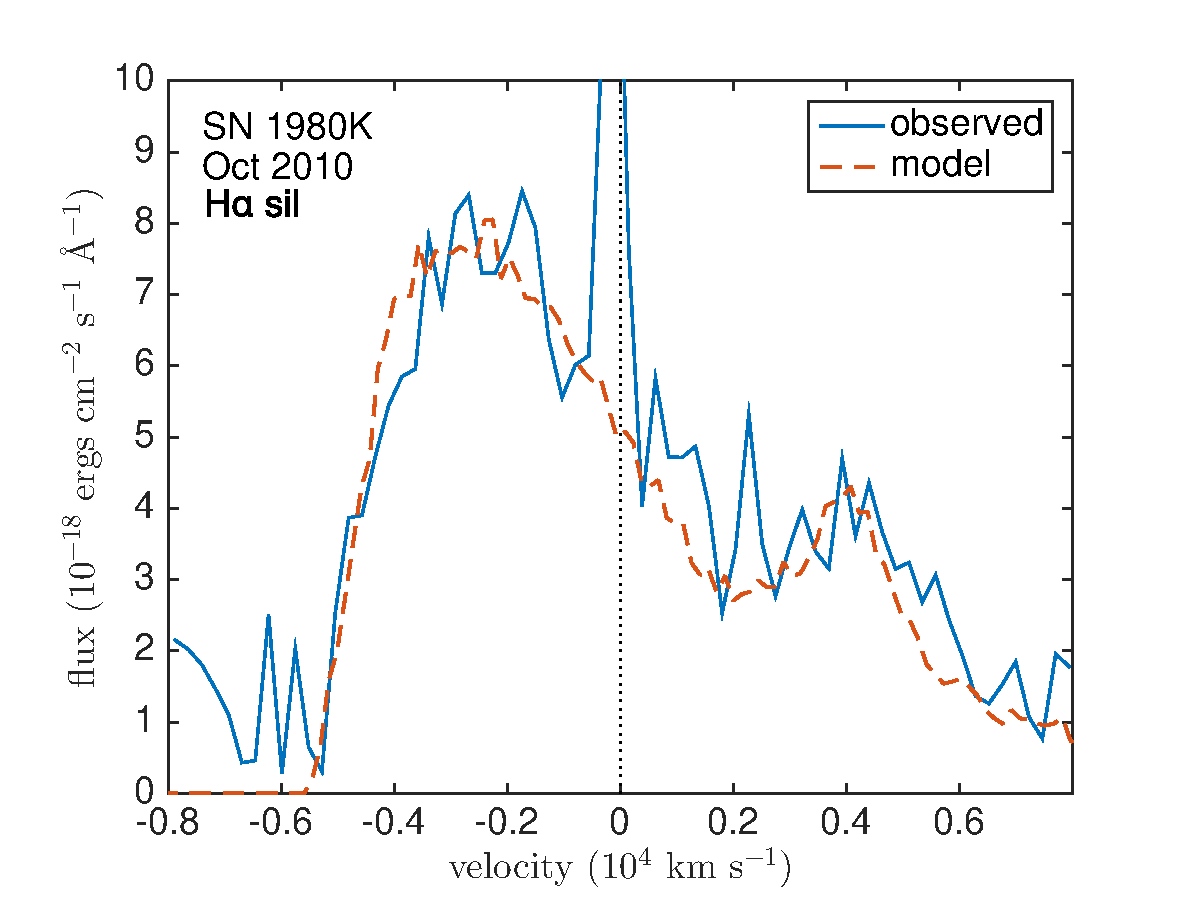
\includegraphics[scale=0.4,clip=true, trim=20 0 40 20]{chapters/chapter6/figs/80K/smooth/Ha}
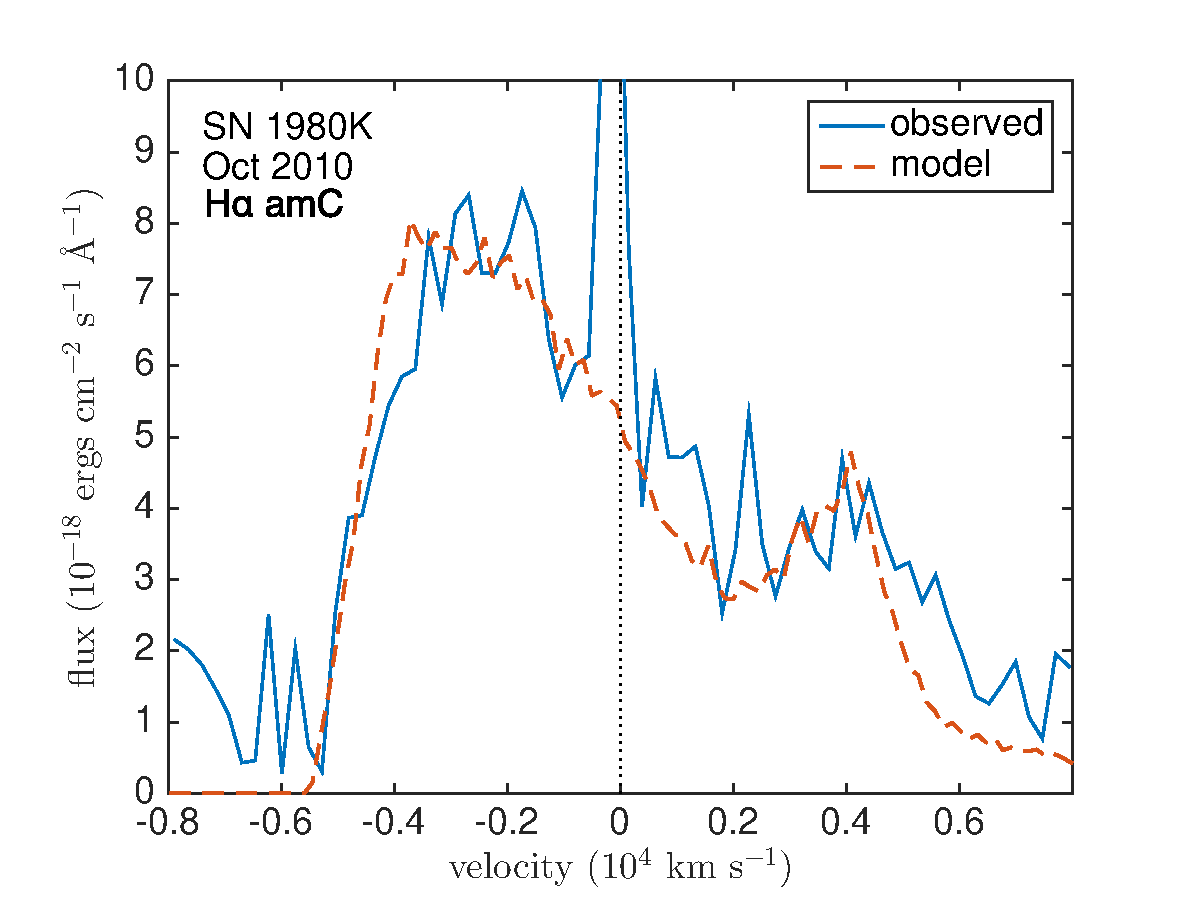
\includegraphics[scale=0.4,clip=true, trim=20 0 40 20]{chapters/chapter6/figs/80K/smooth/Ha_amC}

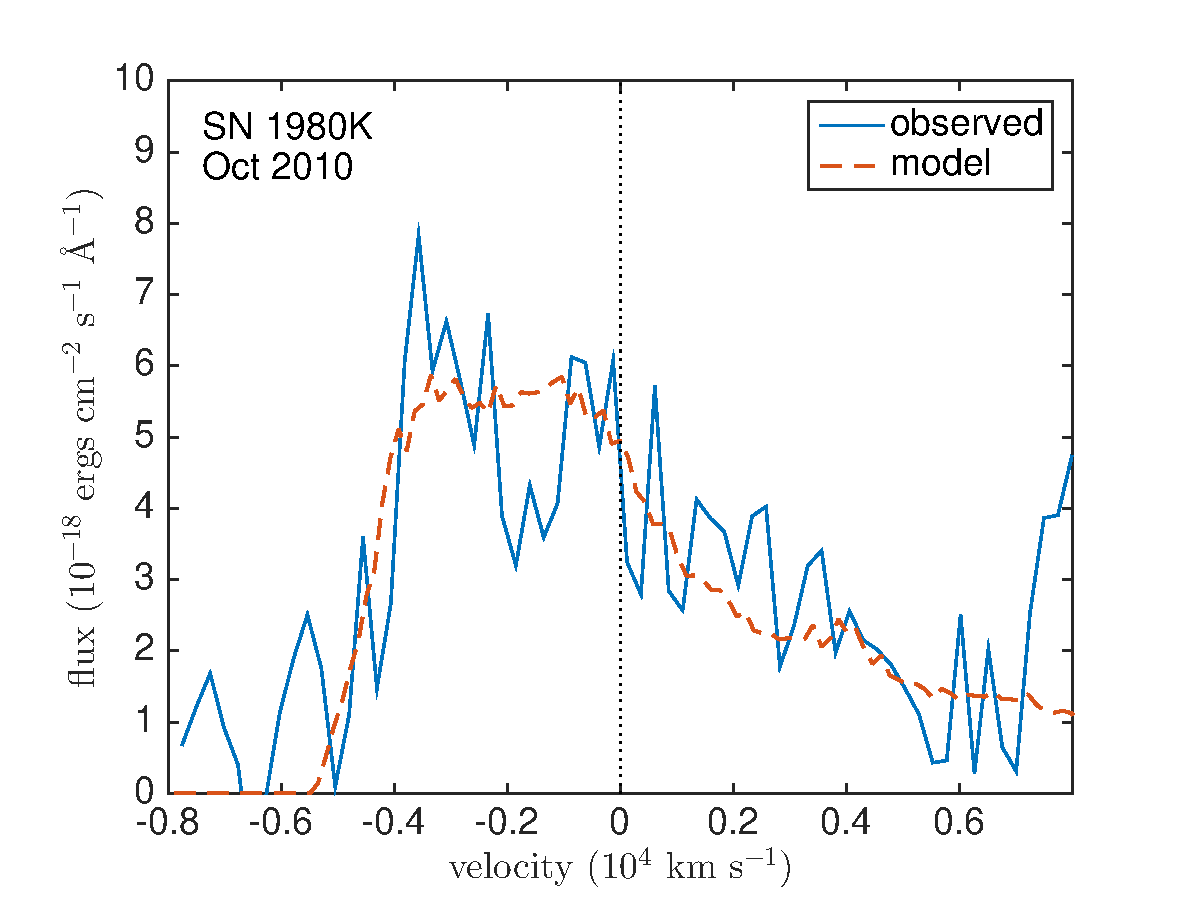
\includegraphics[scale=0.4,clip=true, trim=20 0 40 20]{chapters/chapter6/figs/80K/smooth/OI}
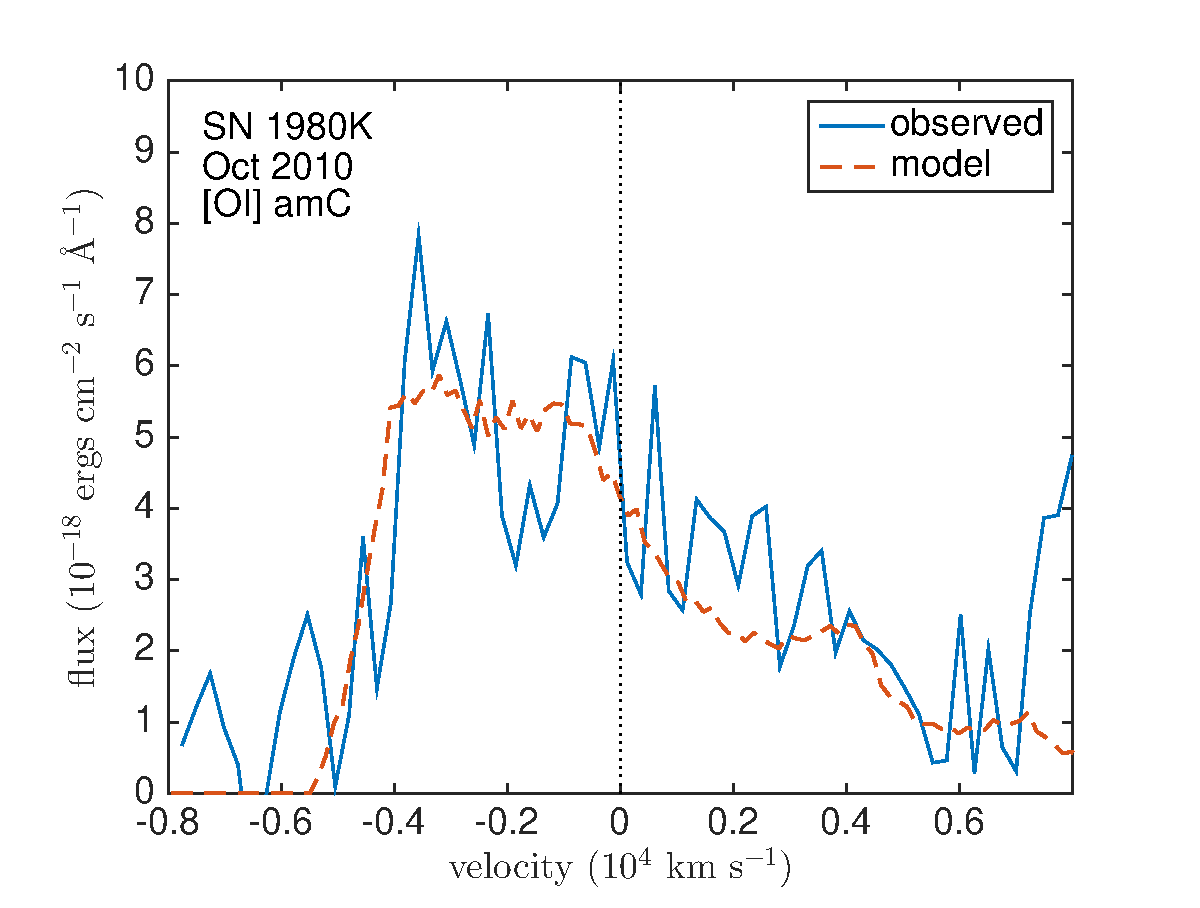
\includegraphics[scale=0.4,clip=true, trim=20 0 40 20]{chapters/chapter6/figs/80K/smooth/OI_amC}
\caption{Smooth fits to SN 1980K}
\label{80K_smooth}
\end{figure}

\begin{figure}
\centering
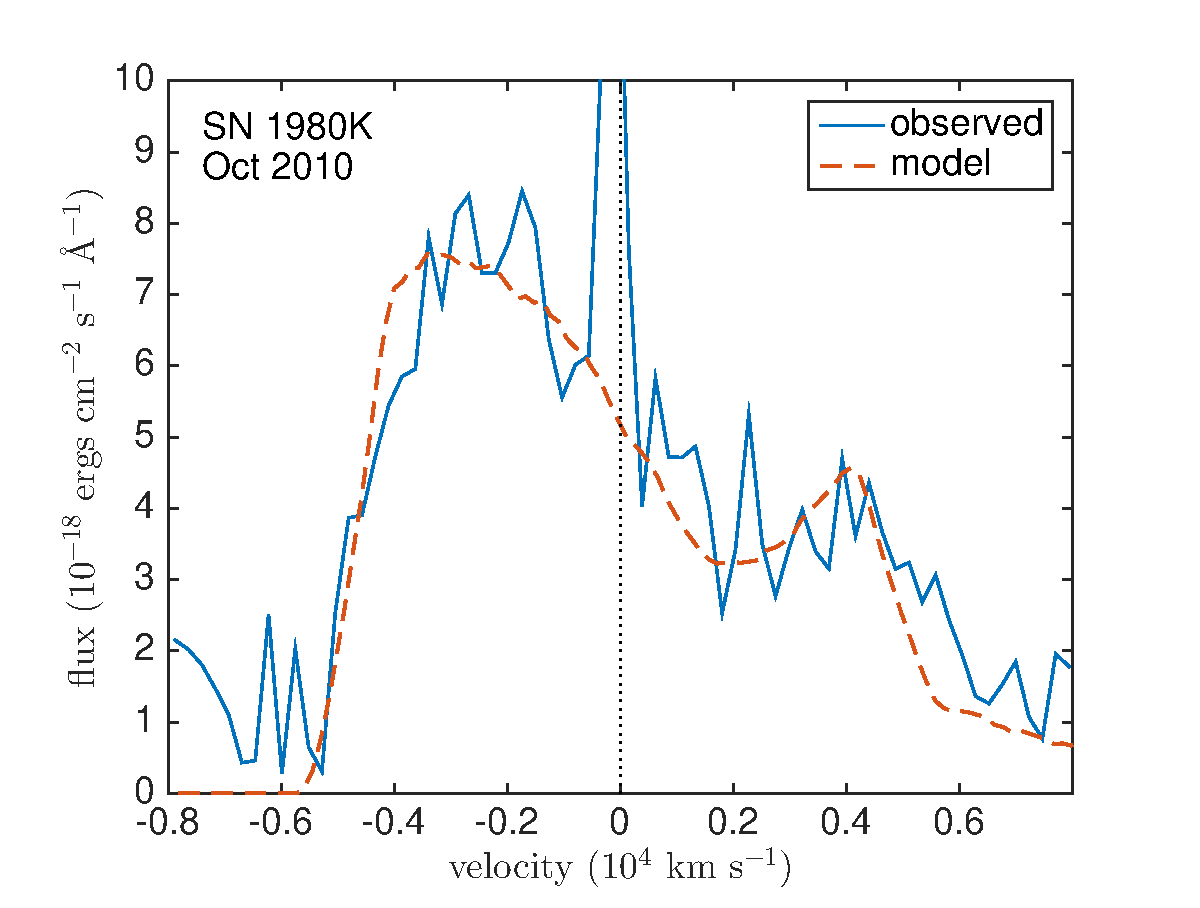
\includegraphics[scale=0.4,clip=true, trim=20 0 40 20]{chapters/chapter6/figs/80K/clumped/Ha}
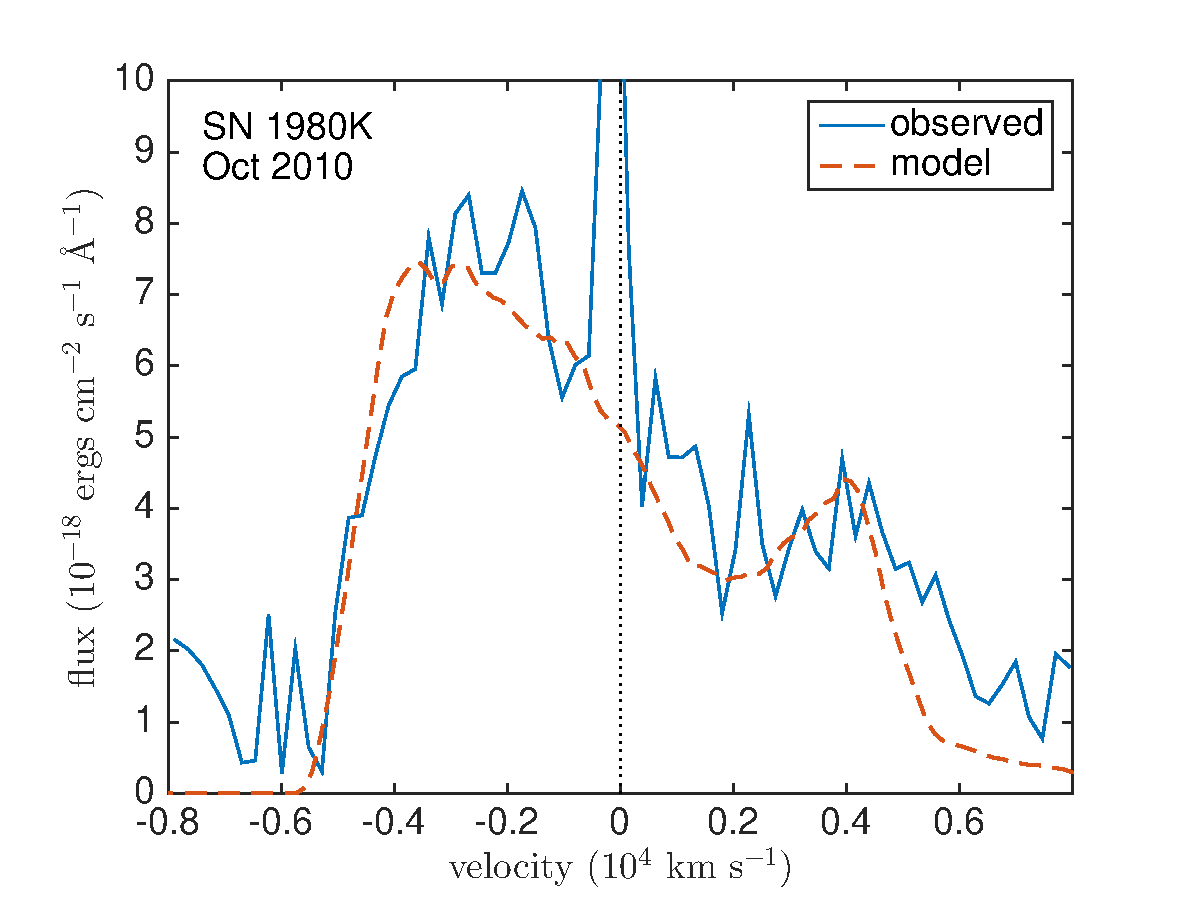
\includegraphics[scale=0.4,clip=true, trim=20 0 40 20]{chapters/chapter6/figs/80K/clumped/Ha_amC}

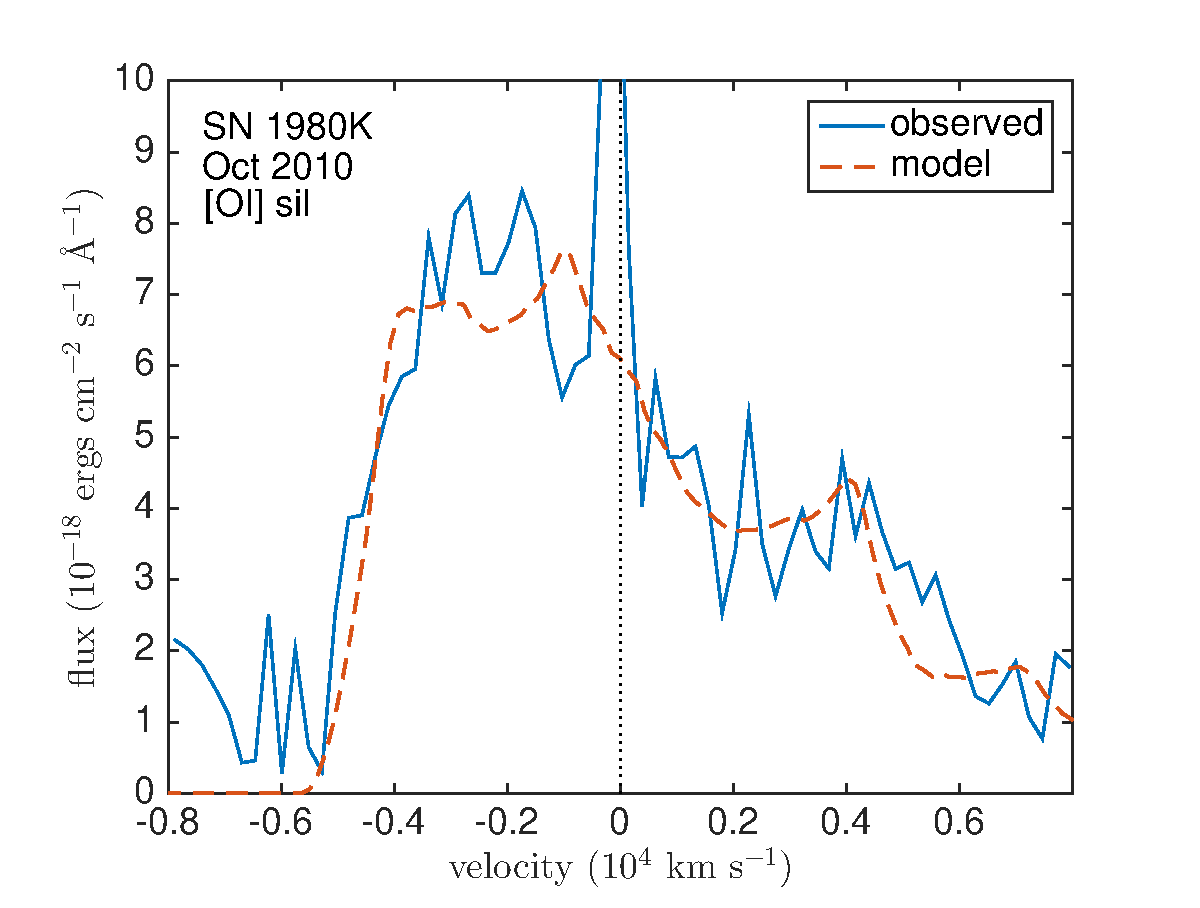
\includegraphics[scale=0.4,clip=true, trim=20 0 40 20]{chapters/chapter6/figs/80K/clumped/OI}
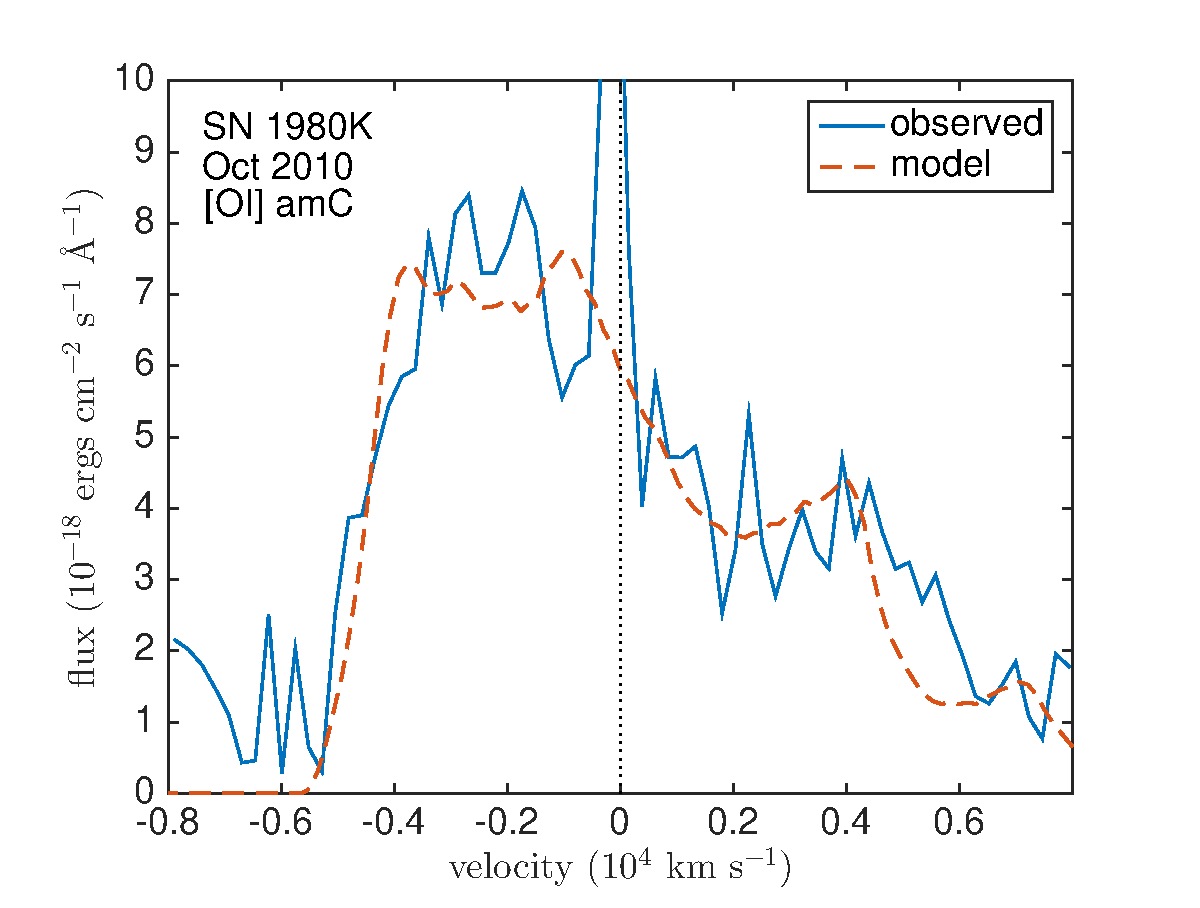
\includegraphics[scale=0.4,clip=true, trim=20 0 40 20]{chapters/chapter6/figs/80K/clumped/OI_amC}
\caption{clumped fits to SN 1980K}
\label{80K_clumped}
\end{figure}

\clearpage

\section{SN~1993J}
\begin{figure}
\centering
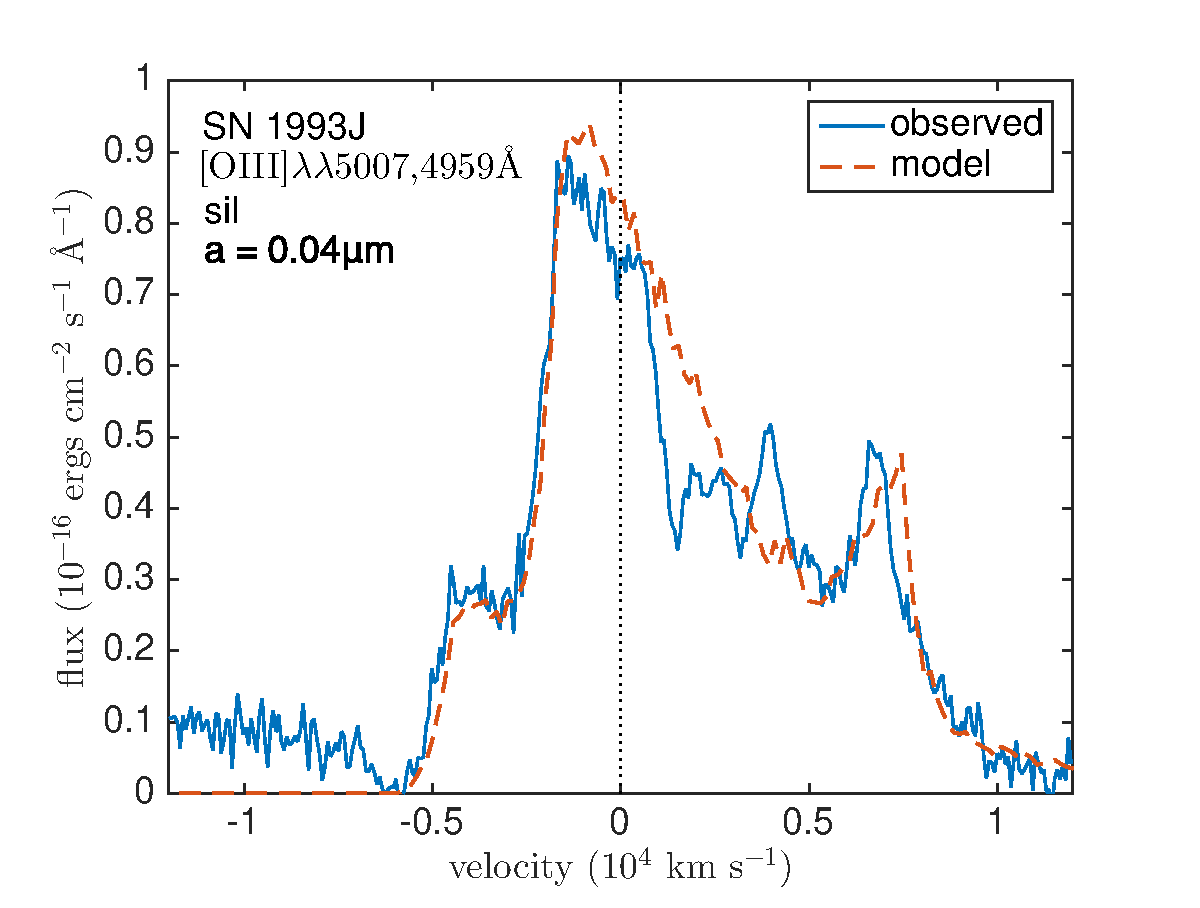
\includegraphics[scale=0.4,clip=true, trim=20 0 40 20]{chapters/chapter6/figs/93J/smooth/OIII}
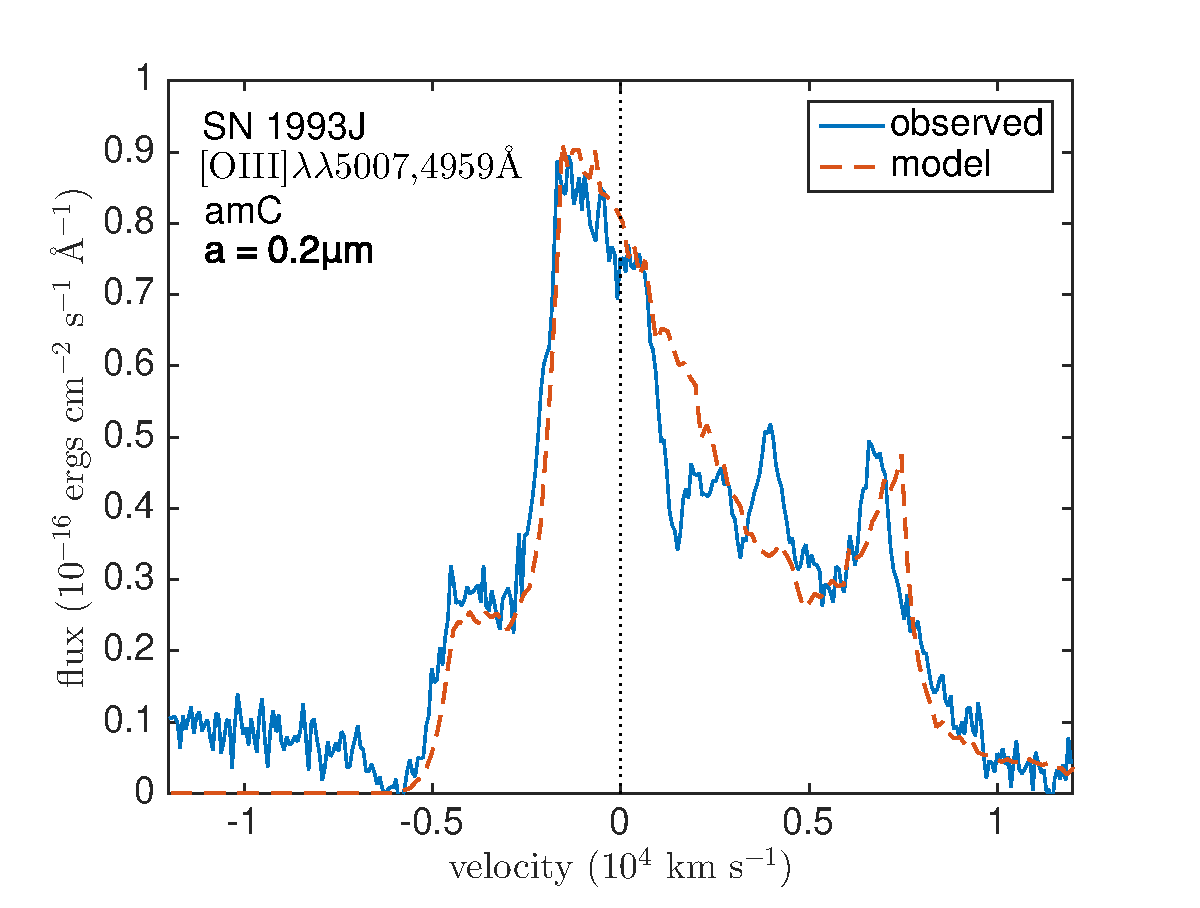
\includegraphics[scale=0.4,clip=true, trim=20 0 40 20]{chapters/chapter6/figs/93J/smooth/OIII_amC}

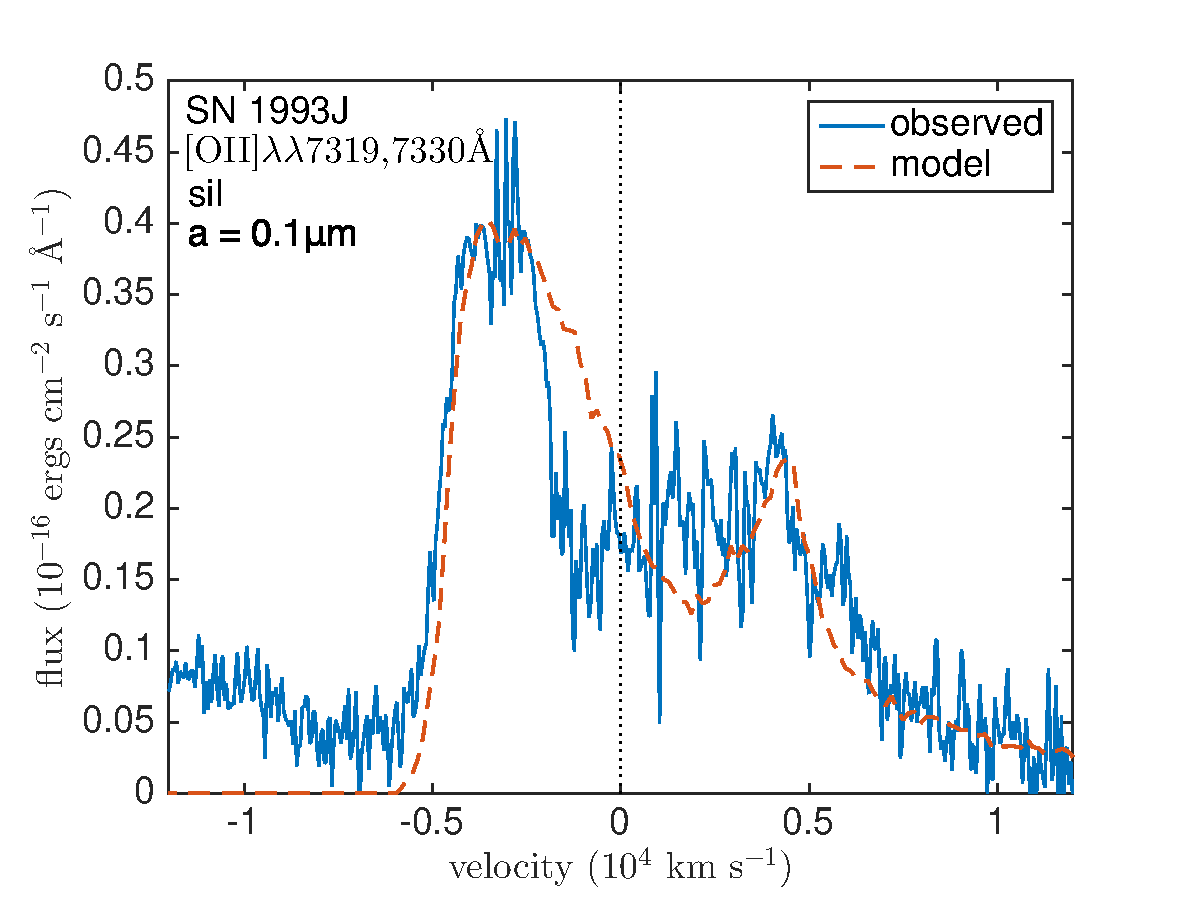
\includegraphics[scale=0.4,clip=true, trim=20 0 40 20]{chapters/chapter6/figs/93J/smooth/OII}
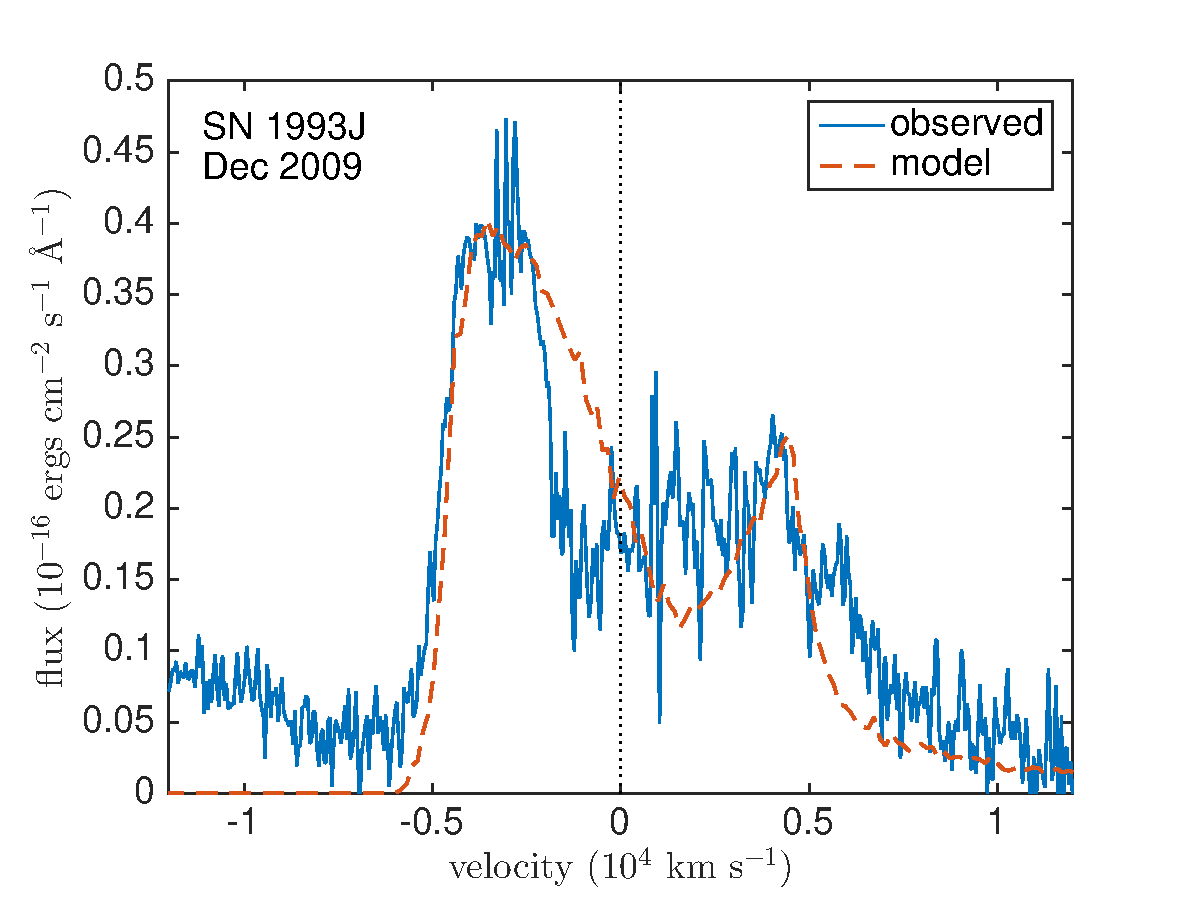
\includegraphics[scale=0.4,clip=true, trim=20 0 40 20]{chapters/chapter6/figs/93J/smooth/OII_amC}
\caption{smooth fits to SN 1993J}
\label{93J_smooth}
\end{figure}

\clearpage

\section{Cassiopeia A}

\begin{figure}
\centering
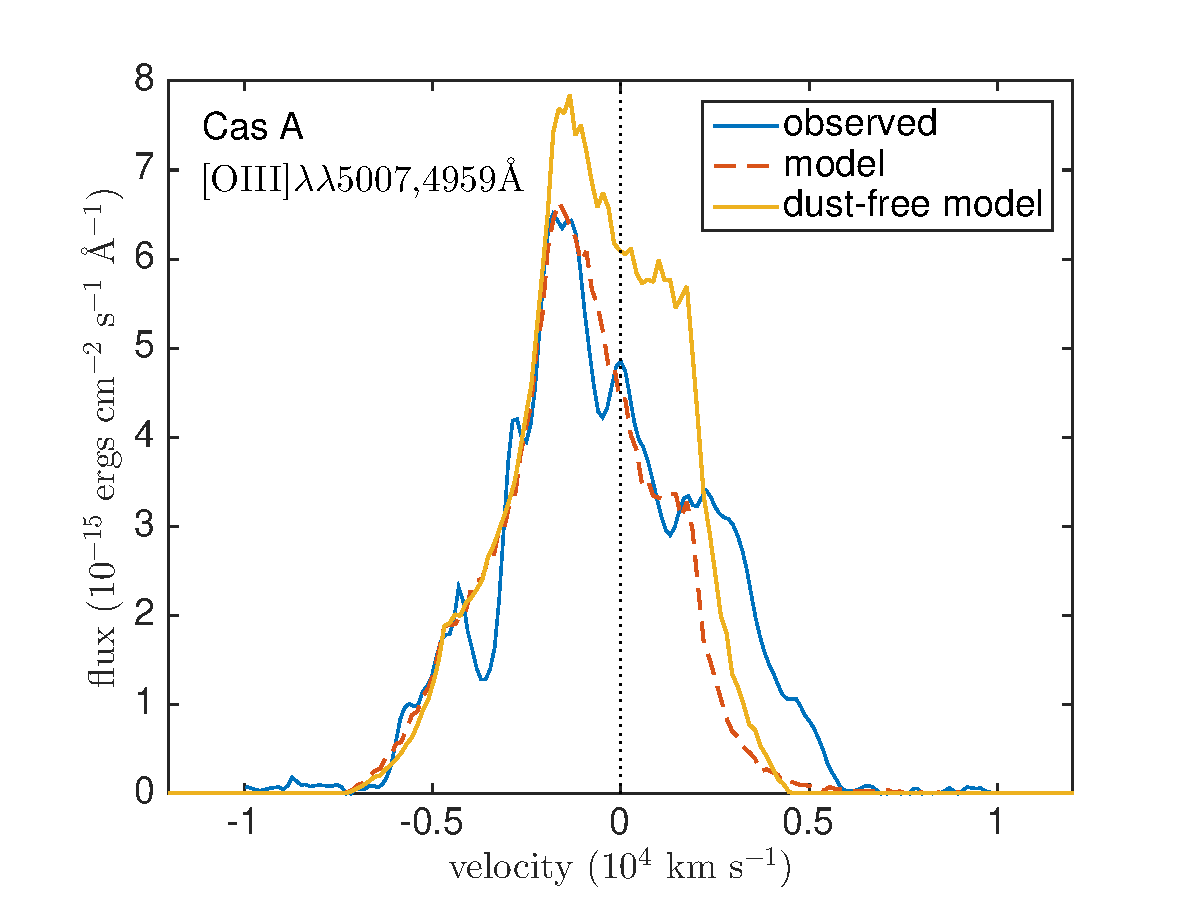
\includegraphics[scale=0.43,clip=true, trim=30 0 50 20]{chapters/chapter6/figs/CasA/CasA_OIII}
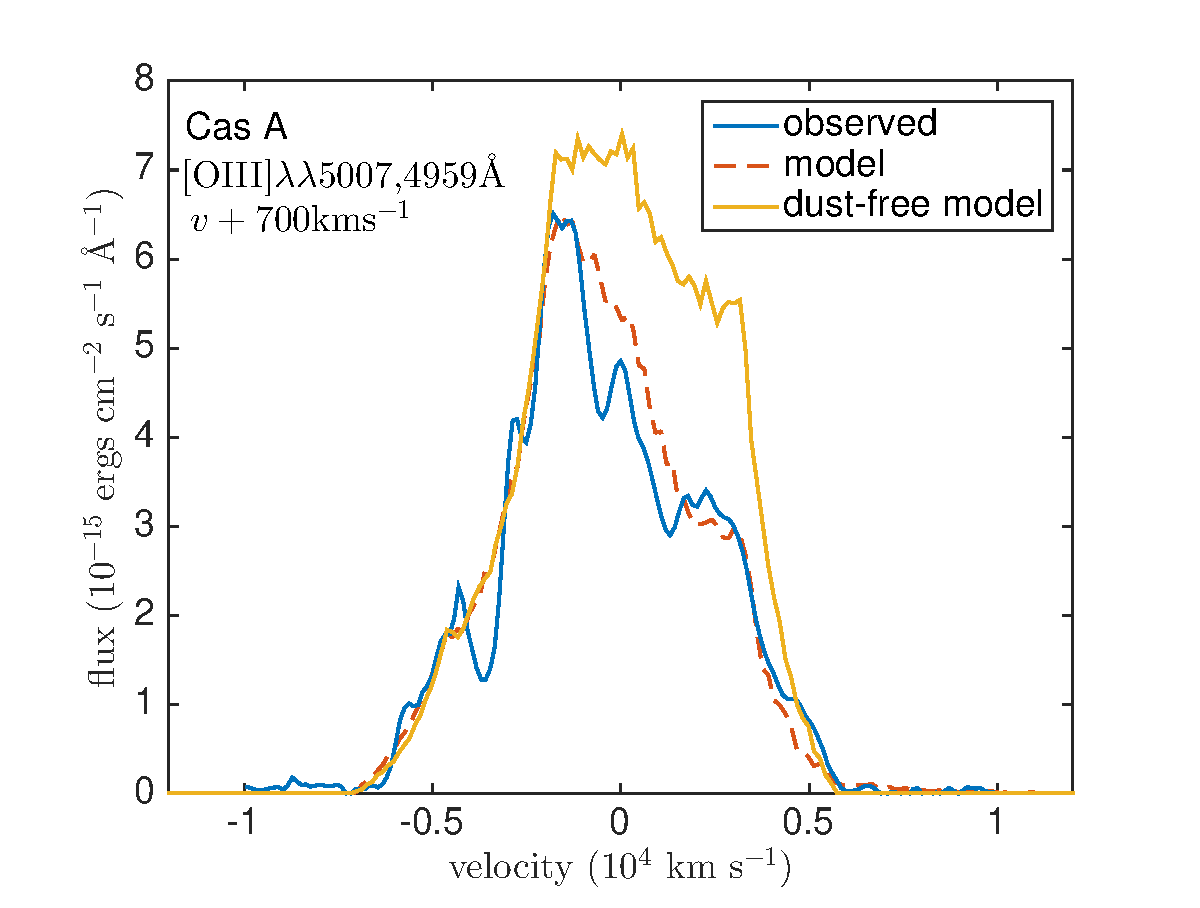
\includegraphics[scale=0.43,clip=true, trim=30 0 50 20]{chapters/chapter6/figs/CasA/CasA_shifted_OIII}
\caption{smooth fits to Cas~A OIII shifted and unshifted}
\label{CasA_OIII}
\end{figure}


\subsection{Smooth Models}

My modelling of the Cas~A spectrum was initially focussed on the [O {\sc iii}] line, which exhibits a pronounced asymmetry.  I managed to produce a reasonable fit to the data using the parameters listed in the first row of Table \ref{CasA_smooth_params}.  The profile is presented in the left pane of Figure \ref{CasA_OIII}.  As can be seen,  the modelled line profile generally fits the observed line profile quite well, although it fails to fit the red side of the profile adequately.  A thorough, manual investigation of parameter space resulted in the conclusion that the profile was much better fitted if the entire observed profile was shifted to the blue by $-700$~km~s$^{-1}$.  This might well be a reasonable assumption.  The integrated spectrum does not sample the entire ejecta.  Additionally, Cas~A is known to be significantly asymmetrical \citep{Rest2011}.  The integrated profile may well sample regions with different line-of-sight velocities, the sum of which could result in a net line-of-sight velocity shift.  This was also found to be the case with the [O {\sc ii}] and [O {\sc i}] lines.  Throughout the remainder of my modelling I therefore allowed the profiles to be shifted in velocity space to better fit the data based on the possibility that the sampled emitting regions had an overall net velocity towards the observer.  Fits to the line profiles were significantly improved following this translation (see Figures \ref{CasA_OIII} to \ref{CasA_clumped_models}).

A model of the shifted [O {\sc iii}] line is presented in Figure \ref{CasA_OIII} and the parameters used for this model are presented in the second row of Table \ref{CasA_smooth_params}.  The line profile was shifted by $-700$~km~s$^{-1}$.  A total dust optical depth of $\tau=0.49$ at 5007\AA\ between $R_{in}$ and $R_{out}$ was found to best fit the profile.  An albedo of $\omega\approx0.15$ at 5007\AA\ was also necessary.

\afterpage{
\begin{landscape}
\setlength{\tabcolsep}{10pt}
\begin{table}
\centering
%	\begin{minipage}{180mm}
	\caption{The parameters used for the smooth models of Cas~A with a medium composed of 50\% amorphous carbon and 50\% silicate grains of radius $a=0.05~\mu$m.  Optical depths are given from $R_{in}$ to $R_{out}$ at $\lambda = 5007$~\AA\ for [O~{\sc iii}], $\lambda = 7319$~\AA\ for [O~{\sc ii}] and $\lambda = 6300$~\AA\ for [O~{\sc i}].  The doublet ratio is always the ratio of the stronger line to the weaker line. The asterisk indicates that the parameters listed describe the gas density distribution.  The dust density distribution is the same in all cases (as detailed for the shifted [O~{\sc ii}] doublet in the second row).}
	\label{CasA_smooth_params}
	\centering
  	\begin{tabular}{@{} cccccccccccc @{}}
    	\hline
  &$v$ shift& $V_{max}$ & $V_{min}$ & $R_{in}/R_{out}$ & $\beta$ & $M_{dust}$ & $R_{out}$ & $R_{in}$ & doublet  & $\tau_{\lambda}$   \\
	& (km~s$^{-1}) $& (km~s$^{-1} $)& (km~s$^{-1} $) & & & ($M_{\odot}$) & (10$^{18}$cm) & (10$^{18}$cm) & ratio \\
	\hline
[O~{\sc iii}]  & 0 & 4500 & 1800 & 0.4  & 2.0 & 1.1 & 4.7 & 1.9 & 2.9 & 0.53  \\ \relax
[O~{\sc iii}]  & -700 & 5000 & 2500 & 0.5  & 2.0 & 1.1 & 5.2 & 2.6 & 2.9 & 0.49  \\ \relax
[O~{\sc ii}]*  & -1000 & 5000 & 3250 & 0.65  & 2.0 & 1.1 & 5.2 & 3.4 & 1.23 & 0.21  \\ \relax
[O~{\sc i}]*  & -1000 & 5000 & 3250 & 0.65  & 2.0 & 1.1 & 5.2 & 3.4 & 3.1 & 0.30  \\ 
    \hline
  \end{tabular}

%\end{minipage}
\end{table}
\end{landscape}
}


The composition of the dust has a significant effect on the overall dust mass for this optical depth and albedo.  A line profile model of the [O {\sc iii}] line profile from Cas~A could not be found using 100\% astronomical silicate dust \citep{Draine1984}.  There is little to no scattering wing seen, hence the relatively low value of $\omega$, and therefore relatively small silicate grains are required to reproduce the red side of the profile.  Silicate grains of this size have extremely low absorption efficiencies and therefore the best-fitting optical depth of $\tau=0.49$ corresponds to an implausibly large mass of dust ($>20$M$_{\odot}$) if it is composed entirely of astronomical silicates.

The chemical composition of the dust in the eject of Cas~A is known to be extremely complex \citep{Arendt2014}.  There are many different species of dust grain present in the ejecta, and it is known that silicate dust is present based on emission features observed in the IR region of the spectrum.  However, the presence of a variety of other species is also predicted.  I therefore investigate the dust masses required to fit the profile for varying fractions of silicate and amorphous carbon dust.  In Table \ref{CasA_dust_masses}, I detail the dust masses required to fit the [O {\sc iii}] line profile for different fractions of silicates and amorphous carbon grains for a single grain size.  For each composition I determine the grain radius based on the albedo necessary to fit the profile ($\omega\approx0.15$) and then vary the dust mass to achieve the required optical depth.  The calculated dust masses cover a wide range of values between 0.65 - 6.5M$_{\odot}$.   All of the line profile models listed above adopted intrinsic doublet strengths from the theory as detailed by \citet{Zeippen1987} and \citet{Storey2000}.  


\begin{figure}
\centering
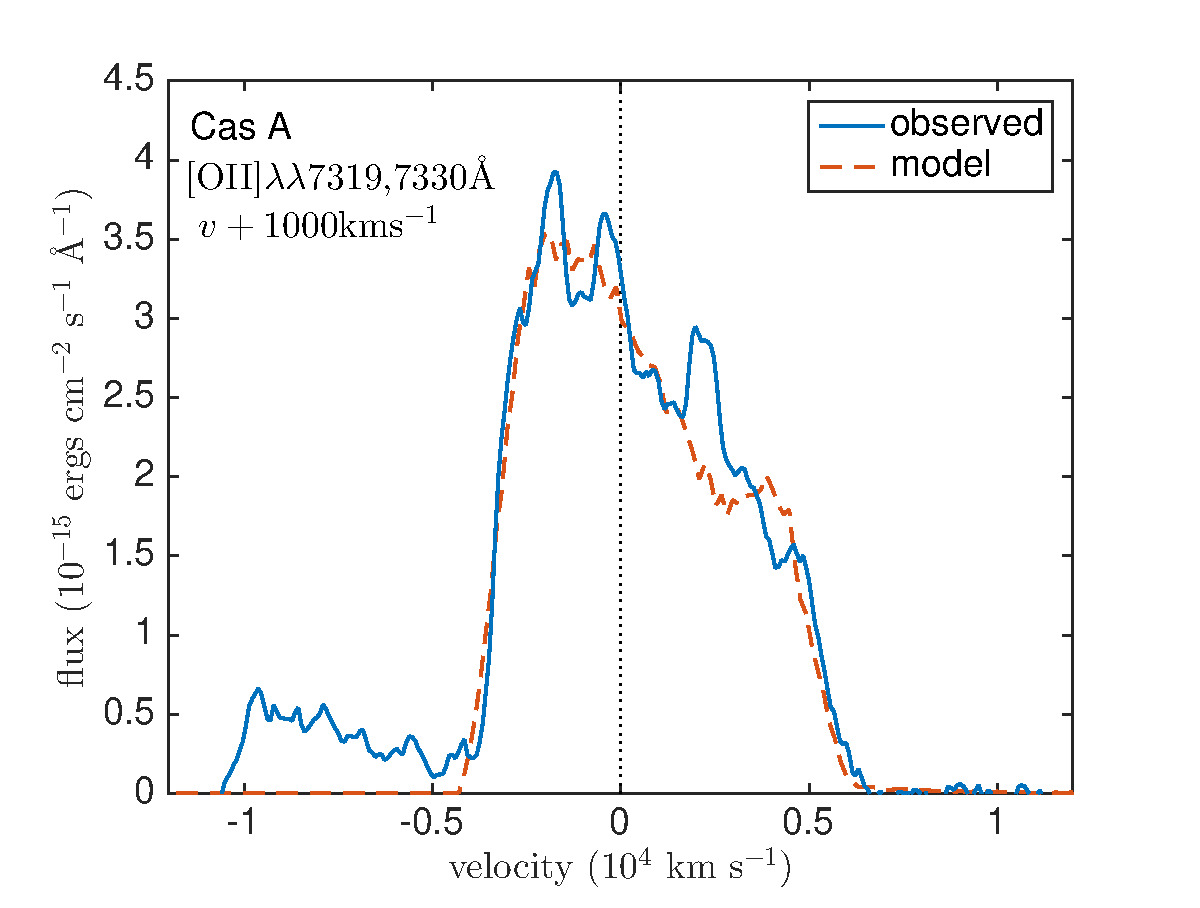
\includegraphics[scale=0.41,clip=true, trim=15 0 40 20]{chapters/chapter6/figs/CasA/CasA_shifted1000_OII}
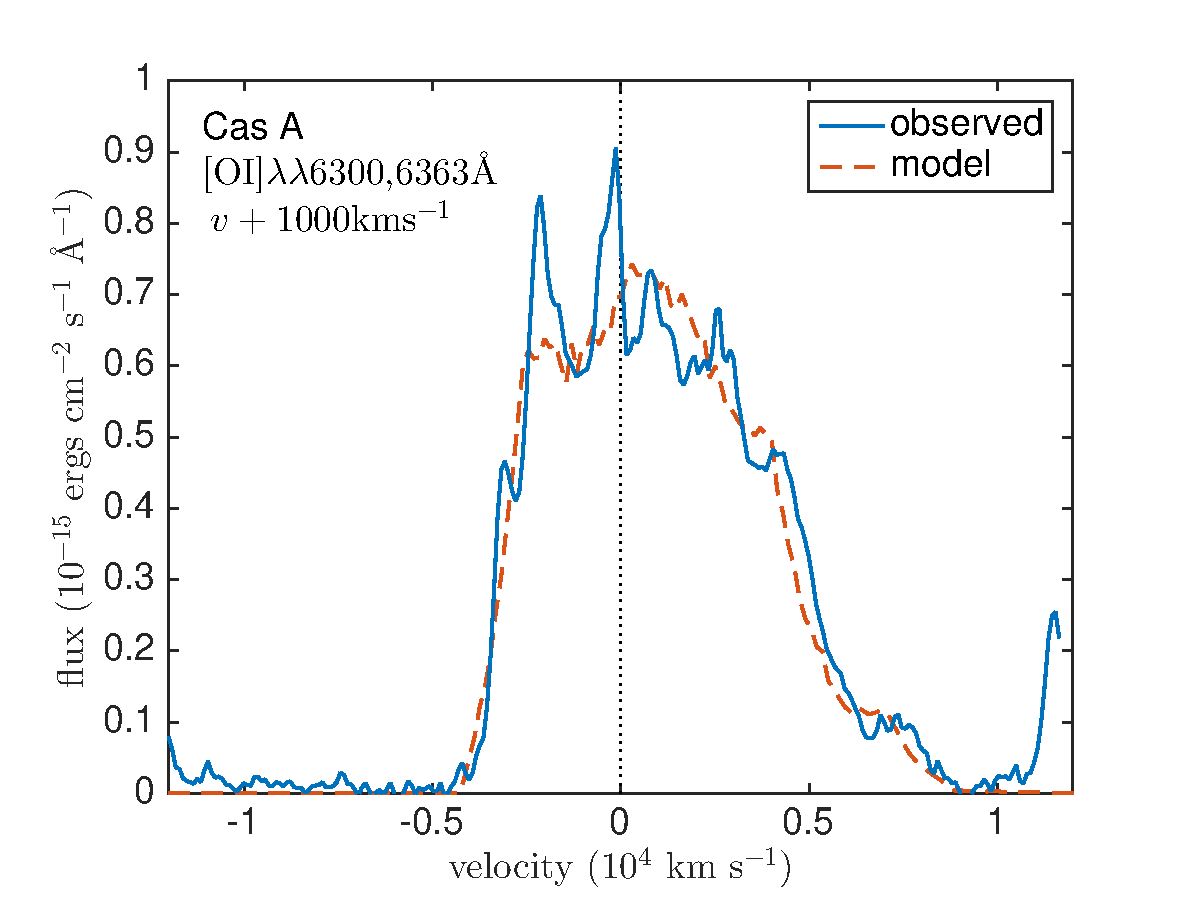
\includegraphics[scale=0.41,clip=true, trim=15 0 40 20]{chapters/chapter6/figs/CasA/CasA_OI_shifted1000}
\caption{Cas~A OI and OII}
\label{CasA_OI_OII}
\end{figure}


\begin{table}
\centering
%	\begin{minipage}{180mm}
	\caption{The variation in dust mass for a fixed optical depth $\tau_{5007\AA}=0.49$ for the parameters listed in Table \ref{CasA_smooth_params}.}
	\label{CasA_dust_masses}
	\centering
  	\begin{tabulary}{12cm}{C C C C}
    	\hline
	\% silicate  & \% amorphous & grain radius $a$ &  $M_{dust}$ \\
	grains& carbon grains&($\mu$m)&(M$_{\odot}$)\\
		\hline
90	&10	&0.035&	6.5 \\
75	&25	&0.04	&2.5\\
50	&50	&0.045&	1.1\\
25	&75	&0.048&	0.6\\
0	&100	&0.05&	0.37\\
    \hline
  \end{tabulary}


\end{table}

It might be possible  to approximately determine the composition based on the relative optical depths necessary to fit different blue-shifted lines in the spectrum and the wavelength dependence of dust absorption for different compositions.  I therefore considered fitting the blue-shifted [O {\sc ii}] and [O {\sc i}] lines from Cas~A.  Sadly, at the small grain sizes required, there is not significant variation in the absorption efficiencies of either amorphous carbon or astronomical silicates between 5007\AA\ and 7319\AA\ and I cannot therefore determine the composition via this approach.  Additionally, the [O {\sc ii}] and [O {\sc i}] lines are much less sensitive to variations in both distribution and dust mass, partly due to the high frequency of bumpy features observed in these lines which contaminate the intrinsic broad profile.  The best-fitting models for these lines were therefore quite degenerate i.e. there were multiple sets of parameters that resulted in reasonable fits.  

However, it was possible to use these lines to determine the feasibility of the best-fitting model for the  [O {\sc iii}] line profile.  I adopted the dust distribution that I determined using the [O {\sc iii}] line and investigated models for the [O {\sc ii}] and [O {\sc i}] line profiles to see if this dust distribution were capable of fitting these lines as well.  I adopted an emissivity distribution that was slightly different to the [O {\sc iii}] line (see Table \ref{CasA_smooth_params}) and shifted the observed line profiles by $-1000$~km~s$^{-1}$.  These emissivity distributions were modelled with the dust distribution and mass for the best-fitting smooth [O {\sc iii}] model.  The resultant [O {\sc ii}] and [O {\sc i}] line profiles are very good fits (see Figure \ref{CasA_OI_OII}).  This suggests that the models are consistent and, if the relative abundance of species can be determined, that the dust masses can be well-constrained.

\subsection{Clumped Models of Cas~A}

The ejecta of Cas~A is highly clumped.  Recently, models by \citet{Biscaro2014} have suggested that dust cannot in fact form in the gas phase in the ejecta of Cas~A unless extremely dense knots of material are present.  It is therefore important, as with SN~1897A, to consider the effects of clumping on the line profiles.  I continue to focus on the [O {\sc iii}] line profile from Cas~A and consider the effects of clumping.  Clearly, the ejecta has a complex geometry with many clumps of different sizes and likely different ionisation states and dust species within each and therefore the models we present here only aim to provide some indication of the effects of clumping within the ejecta.  To this end I present a number of models of the [O {\sc iii}] line profile based on the smooth fits that I presented in the previous section.  I consider two different clump sizes, ones with width $R_{out}/25$ and ones with width $R_{out}/10$.  I also consider three different clump volume filling factors $f=0.05$, $f=0.1$ and $f=0.25$.  For each combination of clump size and filling factor I re-evaluate the required increase or decrease in the dust mass over the smooth model.  All other parameters were kept fixed such that the emission was emitted smoothly according to the distribution and geometry described by the parameters listed in Table \ref{CasA_smooth_params}.

\begin{figure}
\centering
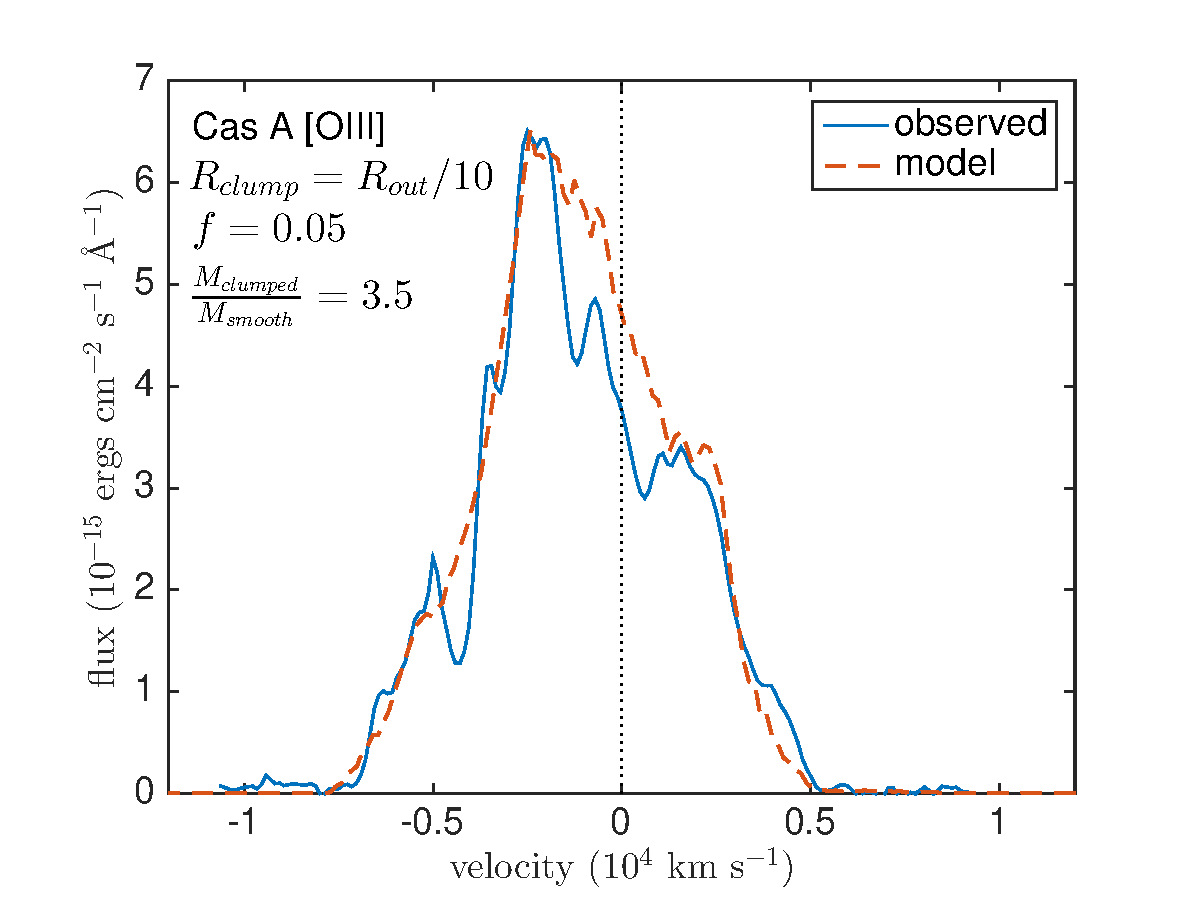
\includegraphics[scale=0.43,clip=true, trim=30 0 50 20]{chapters/chapter6/figs/CasA/clumped/CasA_OIII_c10_f0_05}
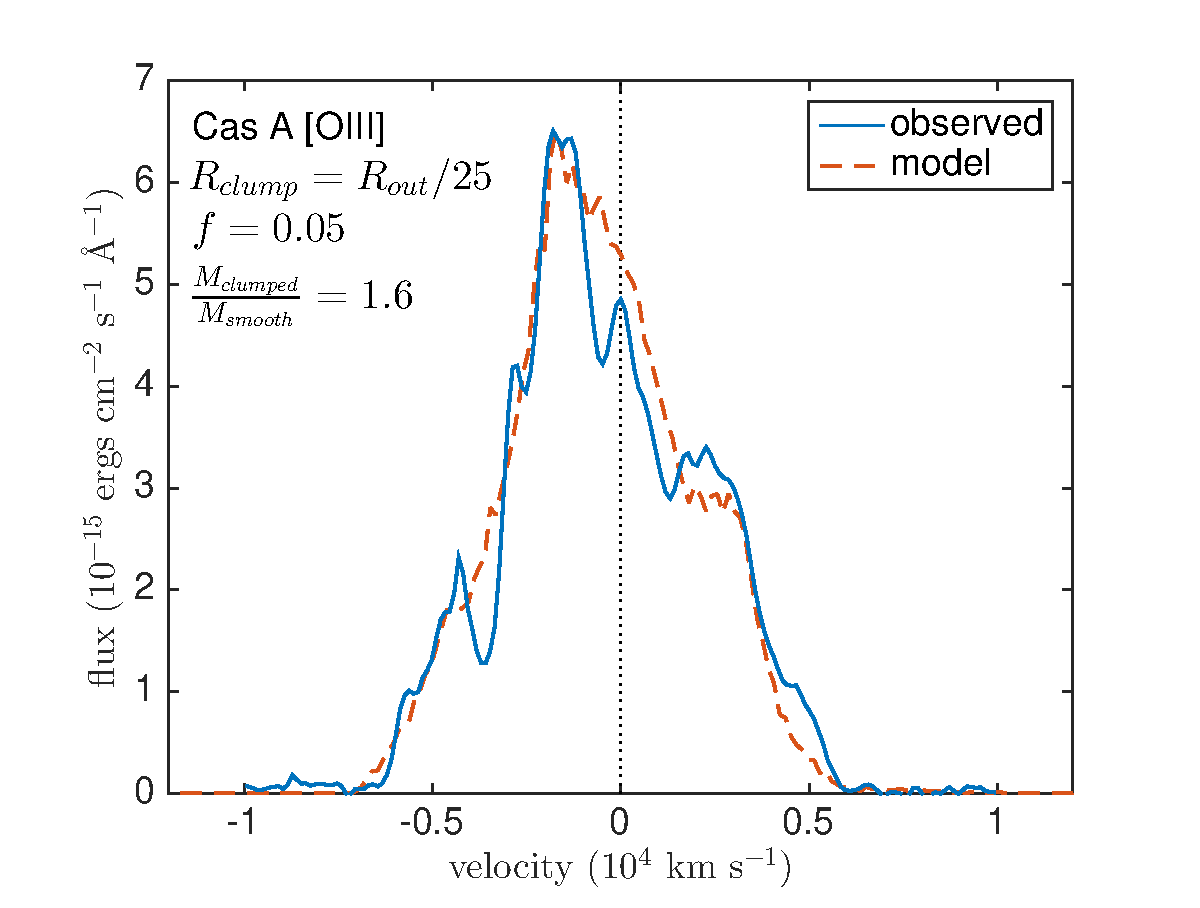
\includegraphics[scale=0.43,clip=true, trim=30 0 40 20]{chapters/chapter6/figs/CasA/clumped/CasA_OIII_c25_f0_05}

\vspace{6mm}
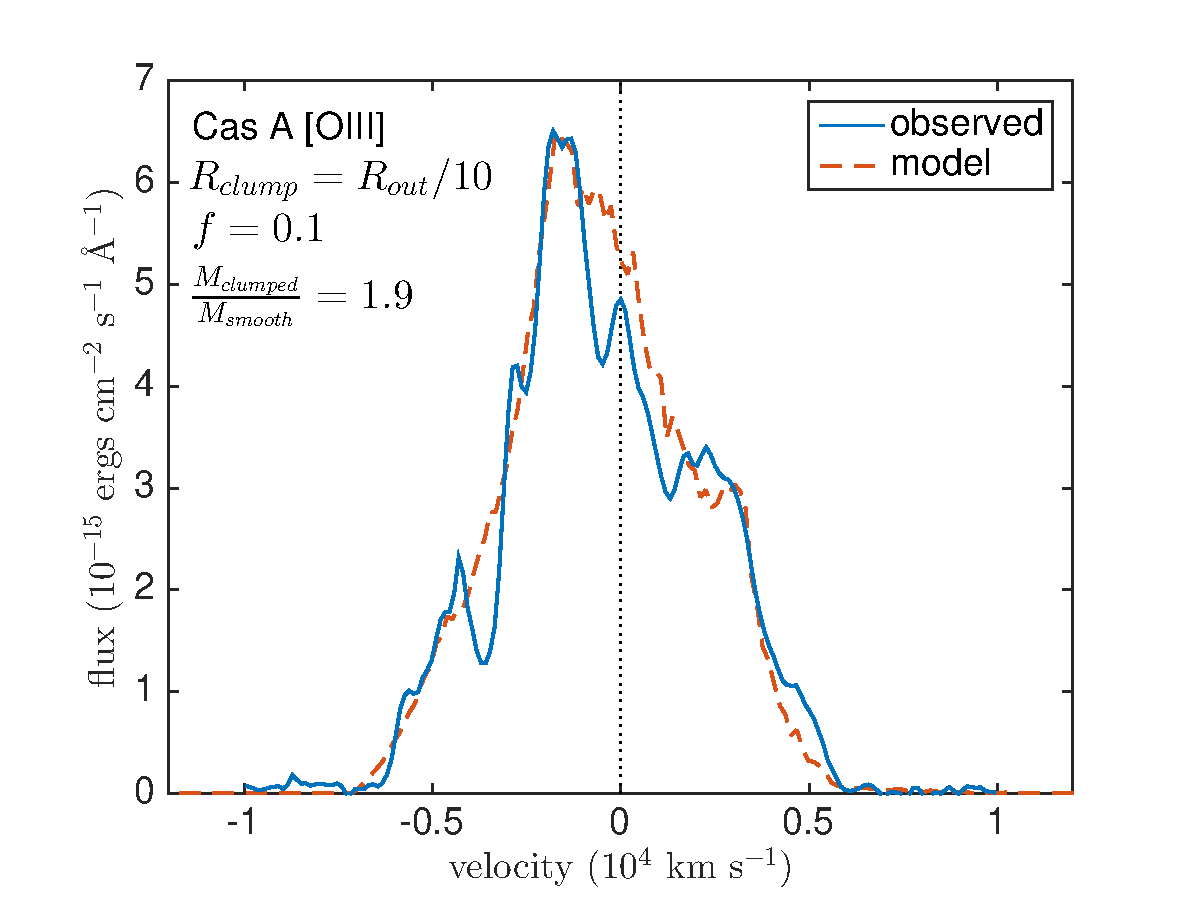
\includegraphics[scale=0.43,clip=true, trim=30 0 50 20]{chapters/chapter6/figs/CasA/clumped/CasA_OIII_c10_f0_1}
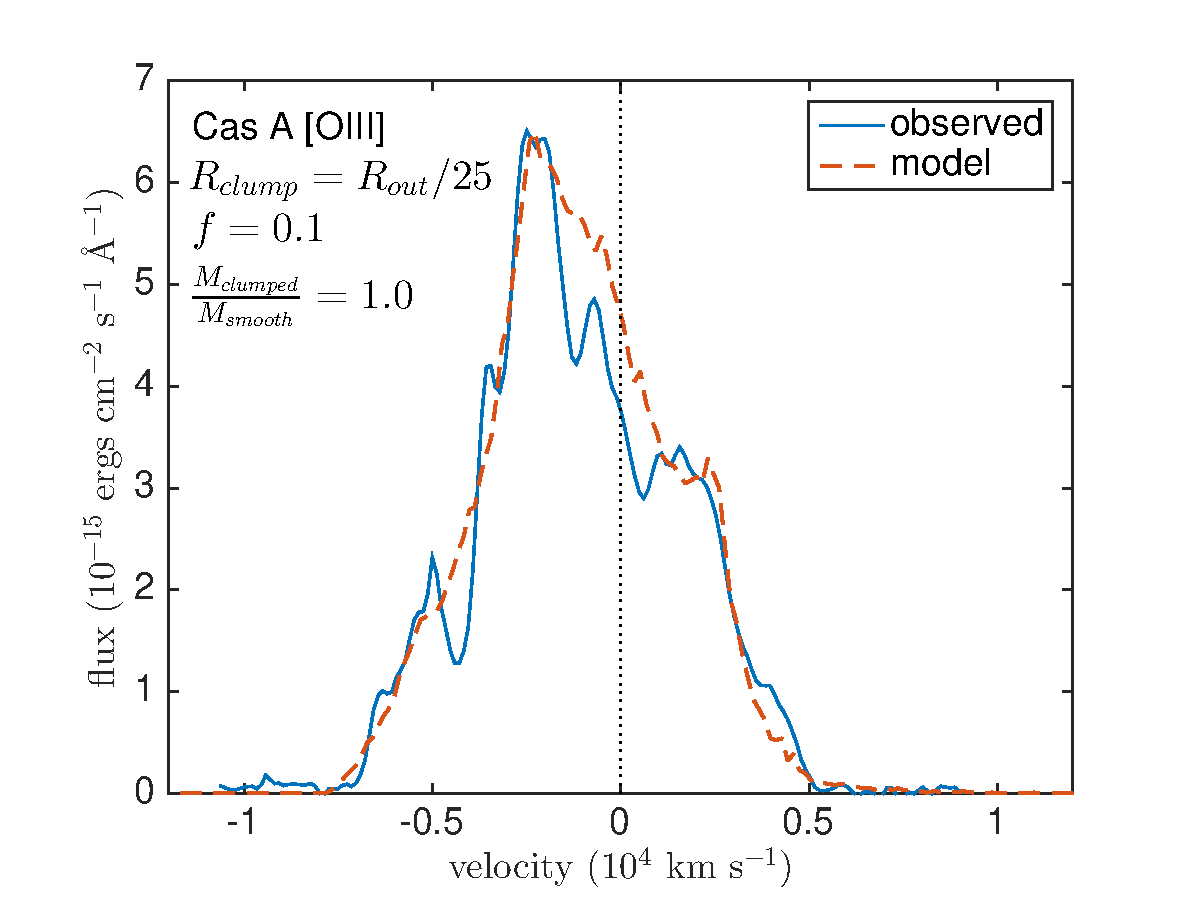
\includegraphics[scale=0.43,clip=true, trim=30 0 40 20]{chapters/chapter6/figs/CasA/clumped/CasA_OIII_c25_f0_1}

\vspace{6mm}
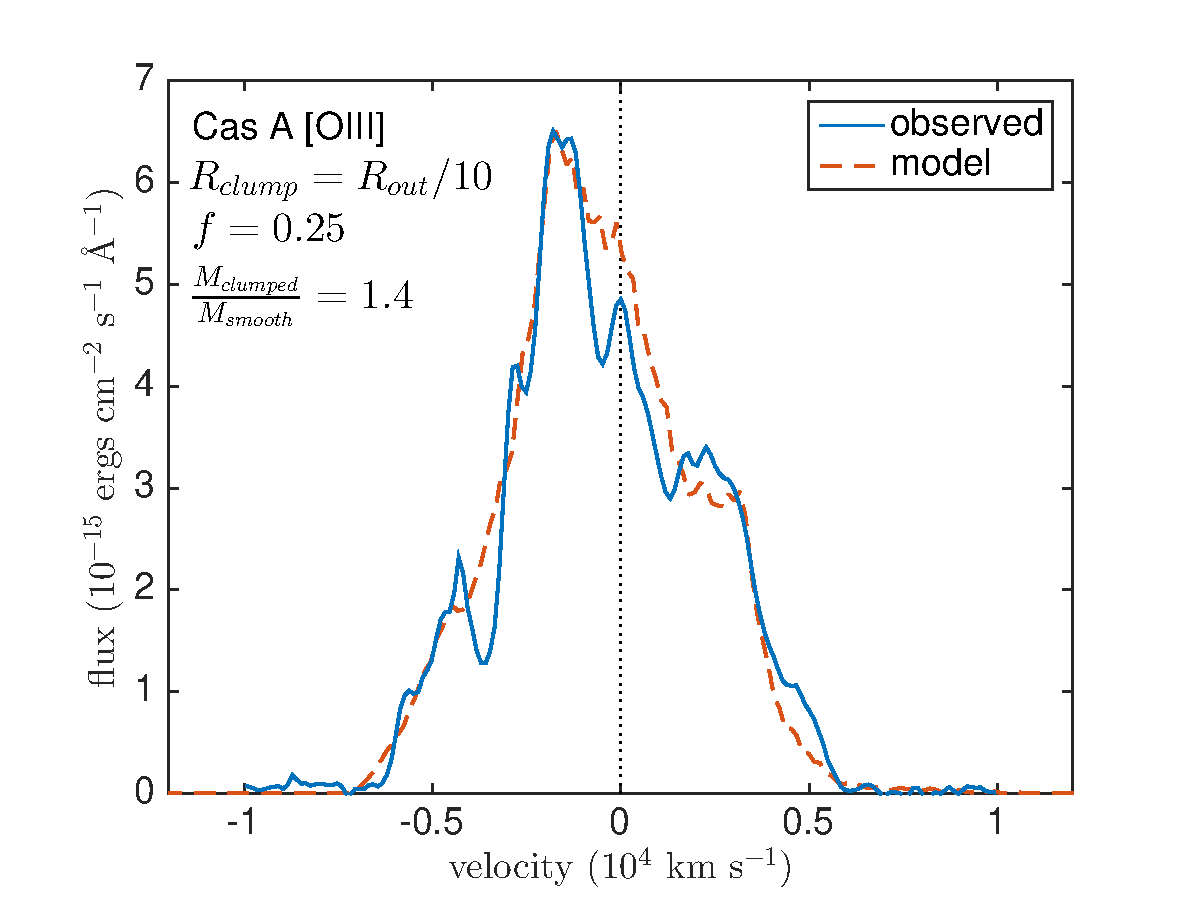
\includegraphics[scale=0.43,clip=true, trim=30 0 50 20]{chapters/chapter6/figs/CasA/clumped/CasA_OIII_c10_f0_25}
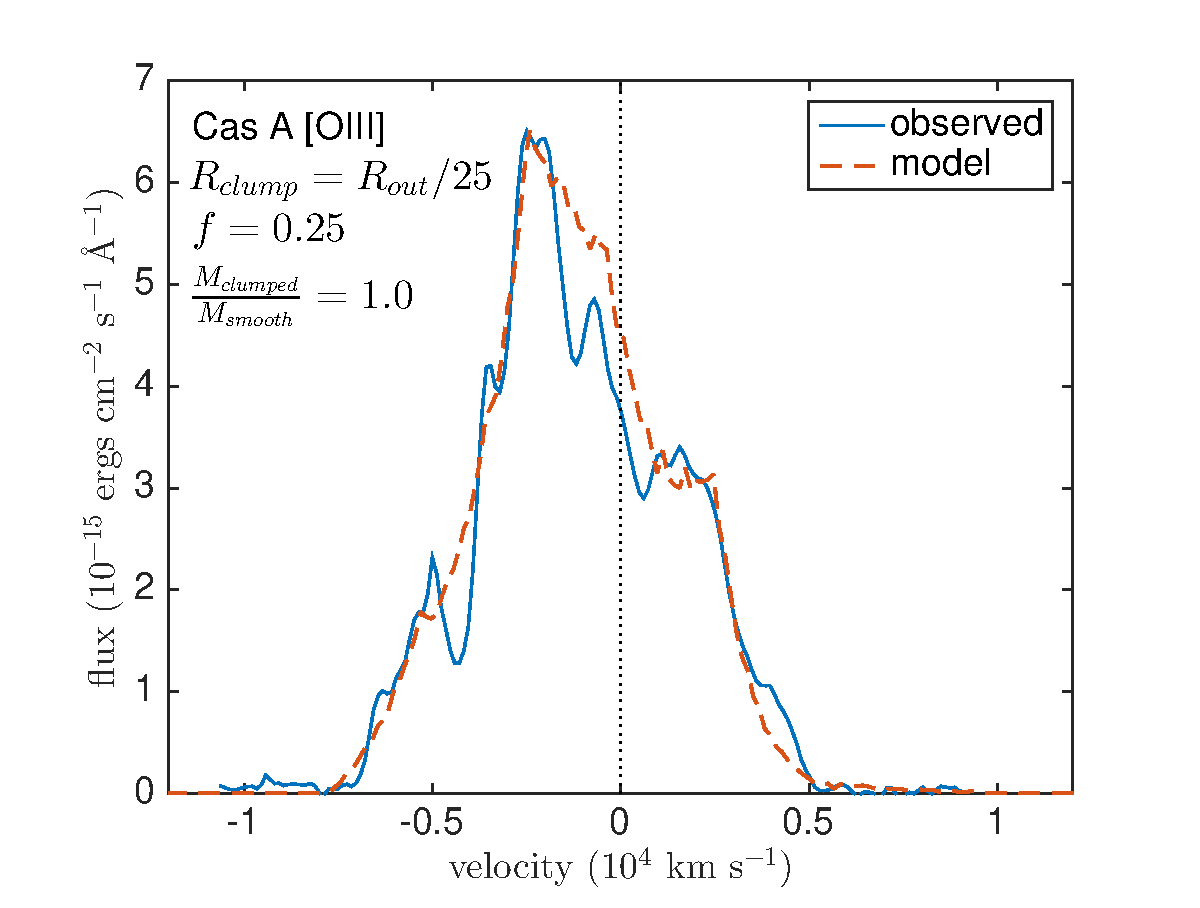
\includegraphics[scale=0.43,clip=true, trim=30 0 40 20]{chapters/chapter6/figs/CasA/clumped/CasA_OIII_c25_f0_25}

\caption{Cas~A clumped}
\label{CasA_OIII_clumped}
\end{figure}

The change in the required dust mass is listed as a fraction of the smooth dust mass (e.g. $M_{dust}=1.1$M$_{\odot}$ for a medium of 50\% astronomical silicates and 50\% amorphous carbon - see Table \ref{CasA_dust_masses} for other dust masses with different dust compositions) is given in Table \ref{CasA_clumped_dust_masses}.  Whilst clumping can be seen to increase the required dust mass in all cases, in the most extreme it is still only by a factor of 3.5.  The fits for each of these cases are presented in Figure \ref{CasA_OIII_clumped}.

\begin{table}
\caption{The fraction of increase in dust mass over the smooth model with parameters as given in Table \ref{CasA_smooth_params} for clumped models with different clump widths and different clump volume filling factors.  The other parameters in the models were fixed at the values given in Table \ref{CasA_smooth_params}.}
\centering
\begin{tabular}{l  c c c}
\hline
& $f=0.05$ &$f=0.1$&$f=0.25$\\
\hline
$R_{out}/10$ & 3.5 & 1.9 & 1.4 \\
$R_{out}/25$ & 1.6 & 1.0 & 1.0 \\
\hline
\end{tabular}
\label{CasA_clumped_dust_masses}
\end{table}













\section{Discussion}

\begin{figure}
\centering
\fbox{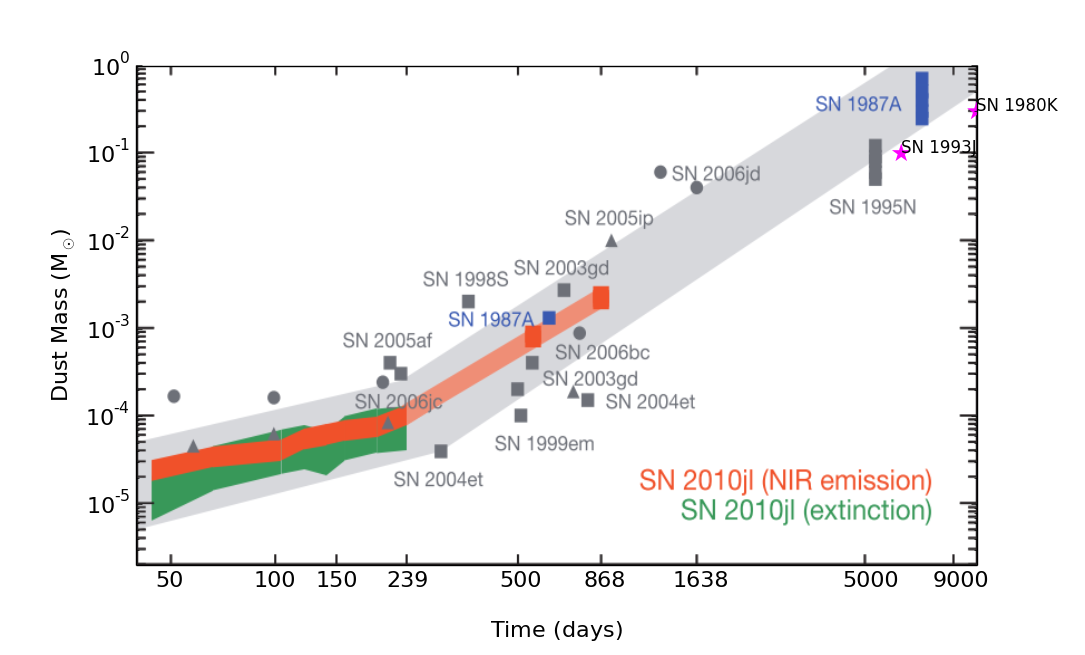
\includegraphics[scale=0.6,clip=true, trim=30 0 0 0]{chapters/chapter6/figs/test.png}}
\caption{dust masses}
\label{shifted}
\end{figure}


\section{Conclusions}
